\section{Appendix: Experiments}
\label{sec:experiments}
\subsection{Results with LoRa}
\label{sec:lora}
\begin{figure}
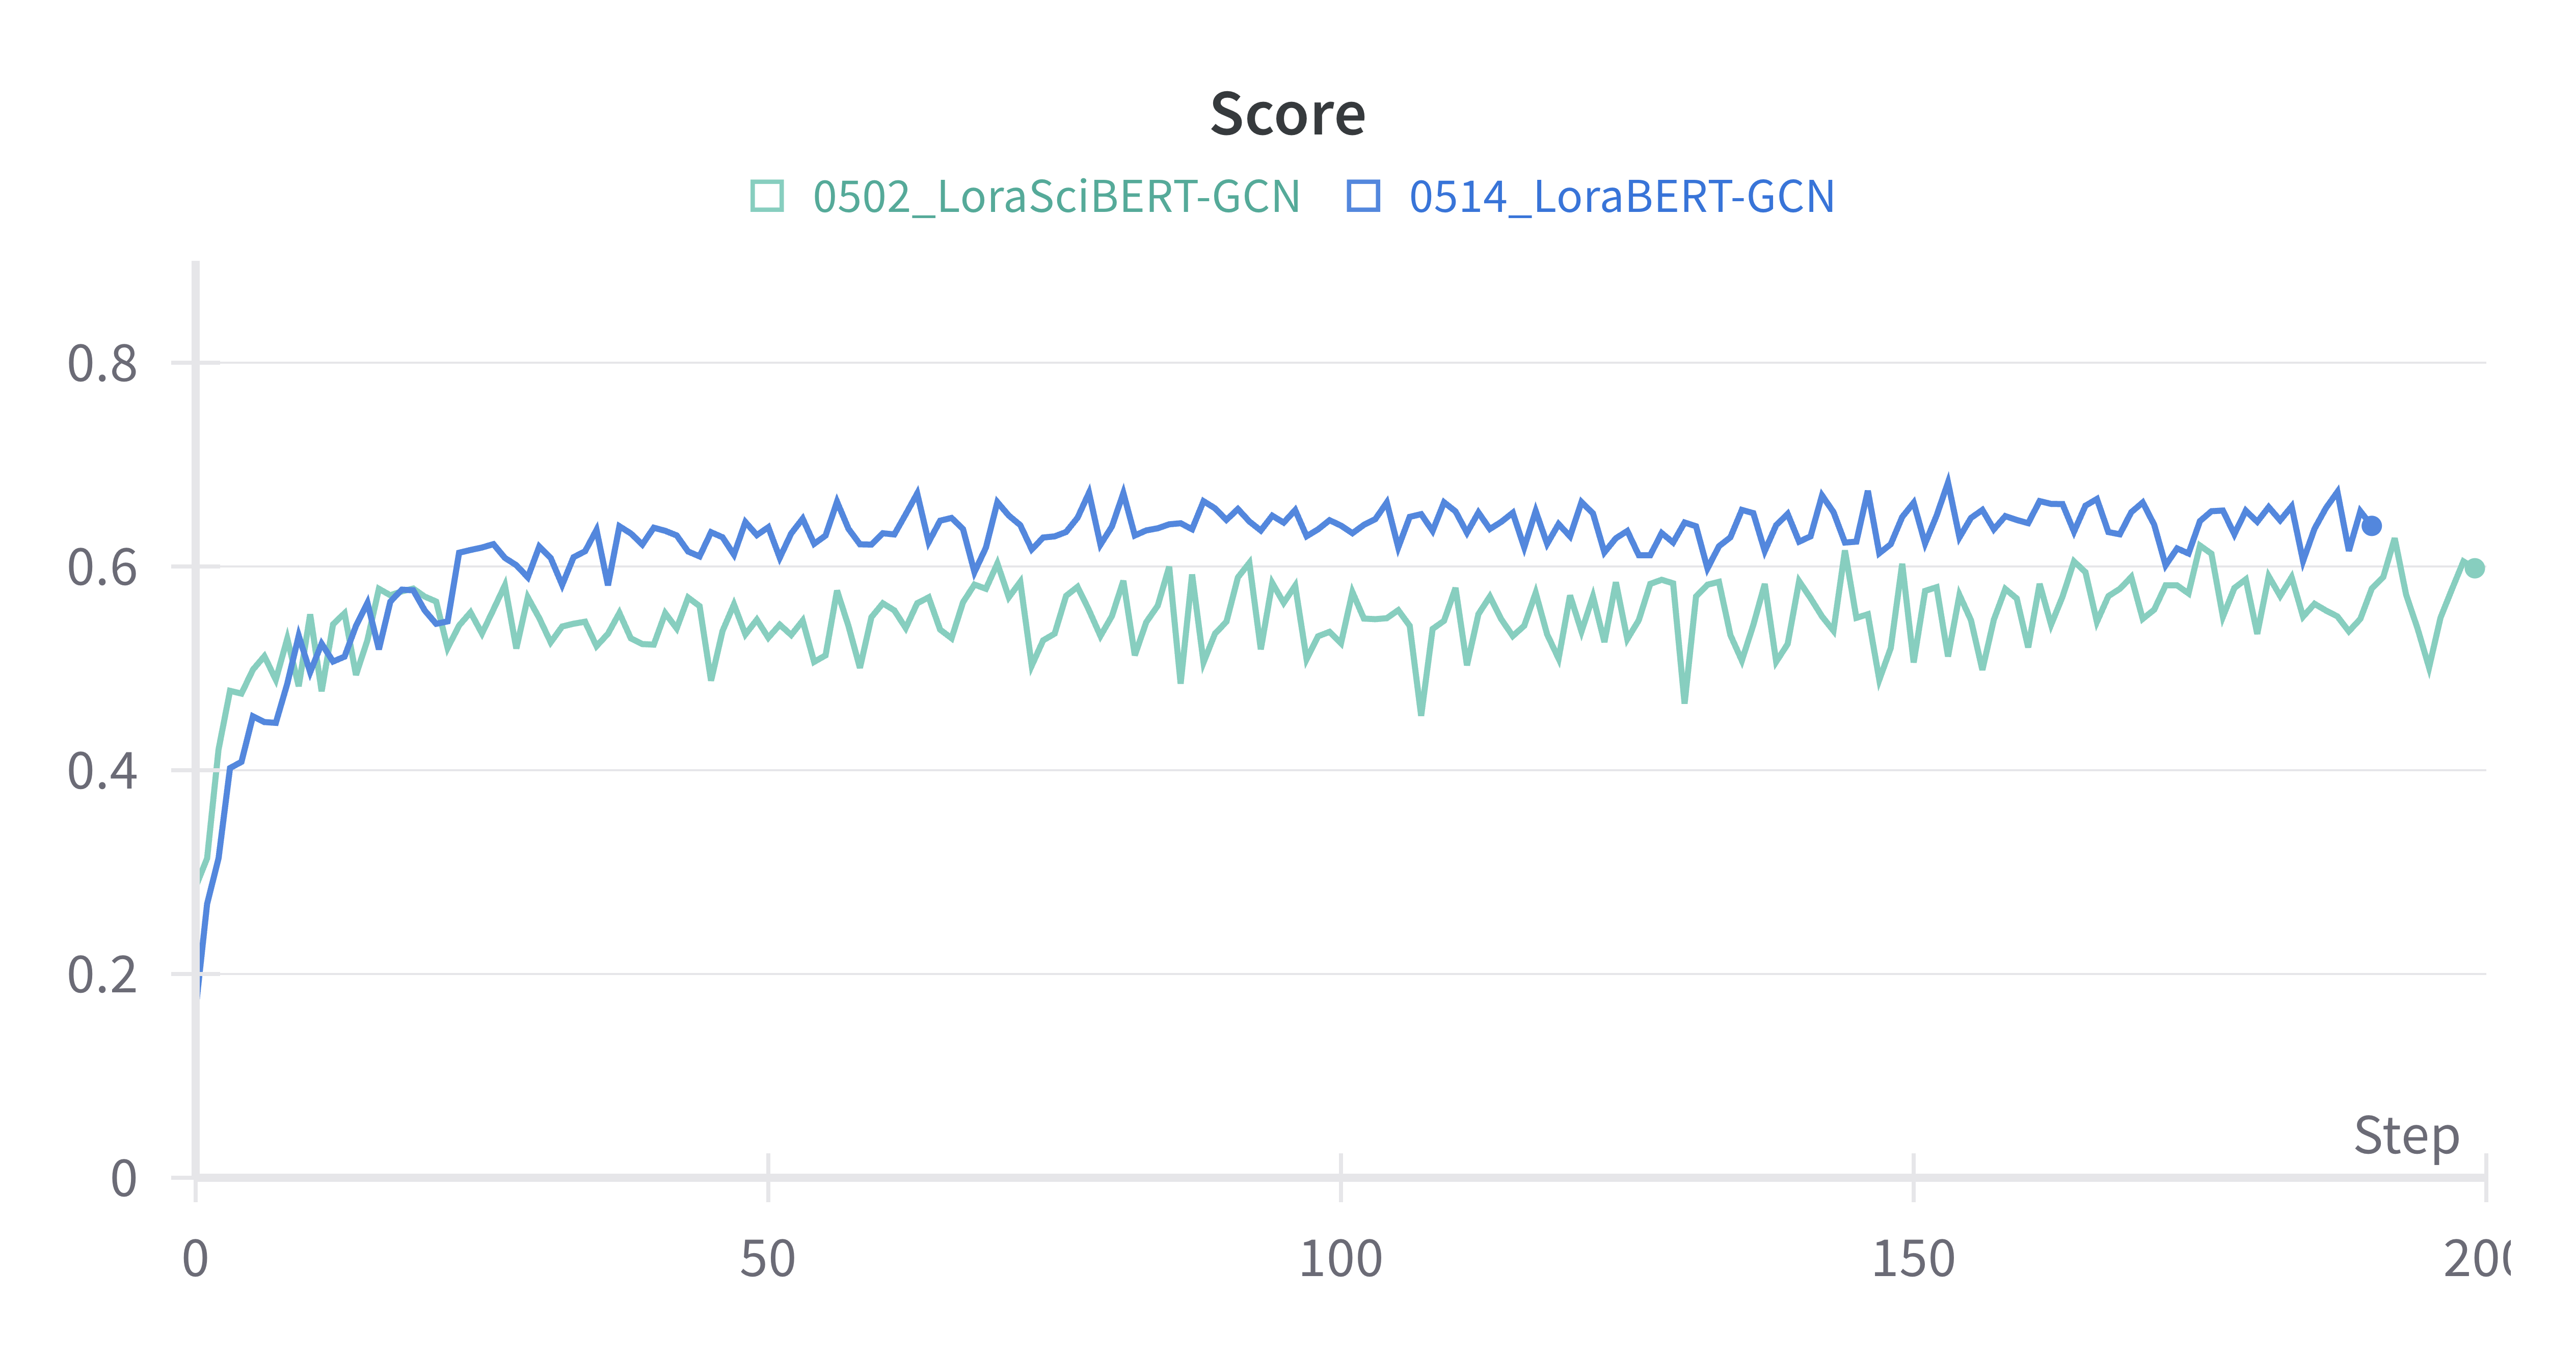
\includegraphics[width=0.3\textwidth]{figures/502_514.png}
\caption{LRAP scores for experiments 502 and 514}
\label{502_fig}
\end{figure}
\begin{table*}[!]
    \centering
    \begin{tabular}{|c|c|c|c|c|c|}
    \hline
    \textbf{Experiment ID} &\textbf{Batch size}& \textbf{Model size} & \textbf{LLM} & \textbf{GNN} & \textbf{LRAP} \\ \hline
    502         &  64    &1.9M & LoRA SciBERT  & Base GCN  & 61.6\%      \\ \hline
     514         &  128    &888k & LoRA BERT  & Base GCN  & 71.8\%      \\ \hline
    \end{tabular}
    \caption{Baseline experiments with LoRA BERT and SciBERT}
    \label{tab:lora}
\end{table*}
We here compare the results of experiments 502 and 514. Their validation scores are displayed on Figure \ref{502_fig}. They were conducted with the same learning rate (3e-4) without a learning rate scheduler. Their specific parameters are detailed in Table \ref{tab:lora}. Memory restrictions keep us from increasing the batch size to 128 in experiment 502.

\subsection{Results for the experiments with different GCN architectures }
\label{sec:gcn}
We compared the influence of the depth of the GCN architecture on several very close models: 502 (base GCN), 571 (big GCN),573 (fat GCN). All elements except for the GCN and the learning scheduler are identical between these experiments. 502 has no learning scheduler which explains the oscillations. We have reason to believe that the Base GCN would have still underperformed compared to 571 and 573 even with the same scheduler. The architecture and parameters of the models are detailed in Table \ref{tab:GCN} and their LRAP scores are displayed on Figure \ref{gcn_fig}
\begin{table*}[!]
    \centering
    \begin{tabular}{|c|c|c|c|c|c|}
    \hline
    \textbf{Experiment ID} &\textbf{Batch size}& \textbf{Model size} & \textbf{LLM} & \textbf{GNN} & \textbf{LRAP} \\ \hline
    502         &  64    &1.9M & LoRA SciBERT  & Base GCN 3 layers & 61.6\%      \\ \hline
     571         &  64    &2.9M & LoRA SciBERT  & Big GCN 5 layers  & 71.6\%      \\ \hline
     573        &  64    &3.4M & LoRA SciBERT  & Fat GCN 7 layers  & 79.6\%      \\ \hline
    \end{tabular}
    \caption{Experiments with LoRa SciBERT and various GCN models}
    \label{tab:GCN}
\end{table*}
\begin{figure}
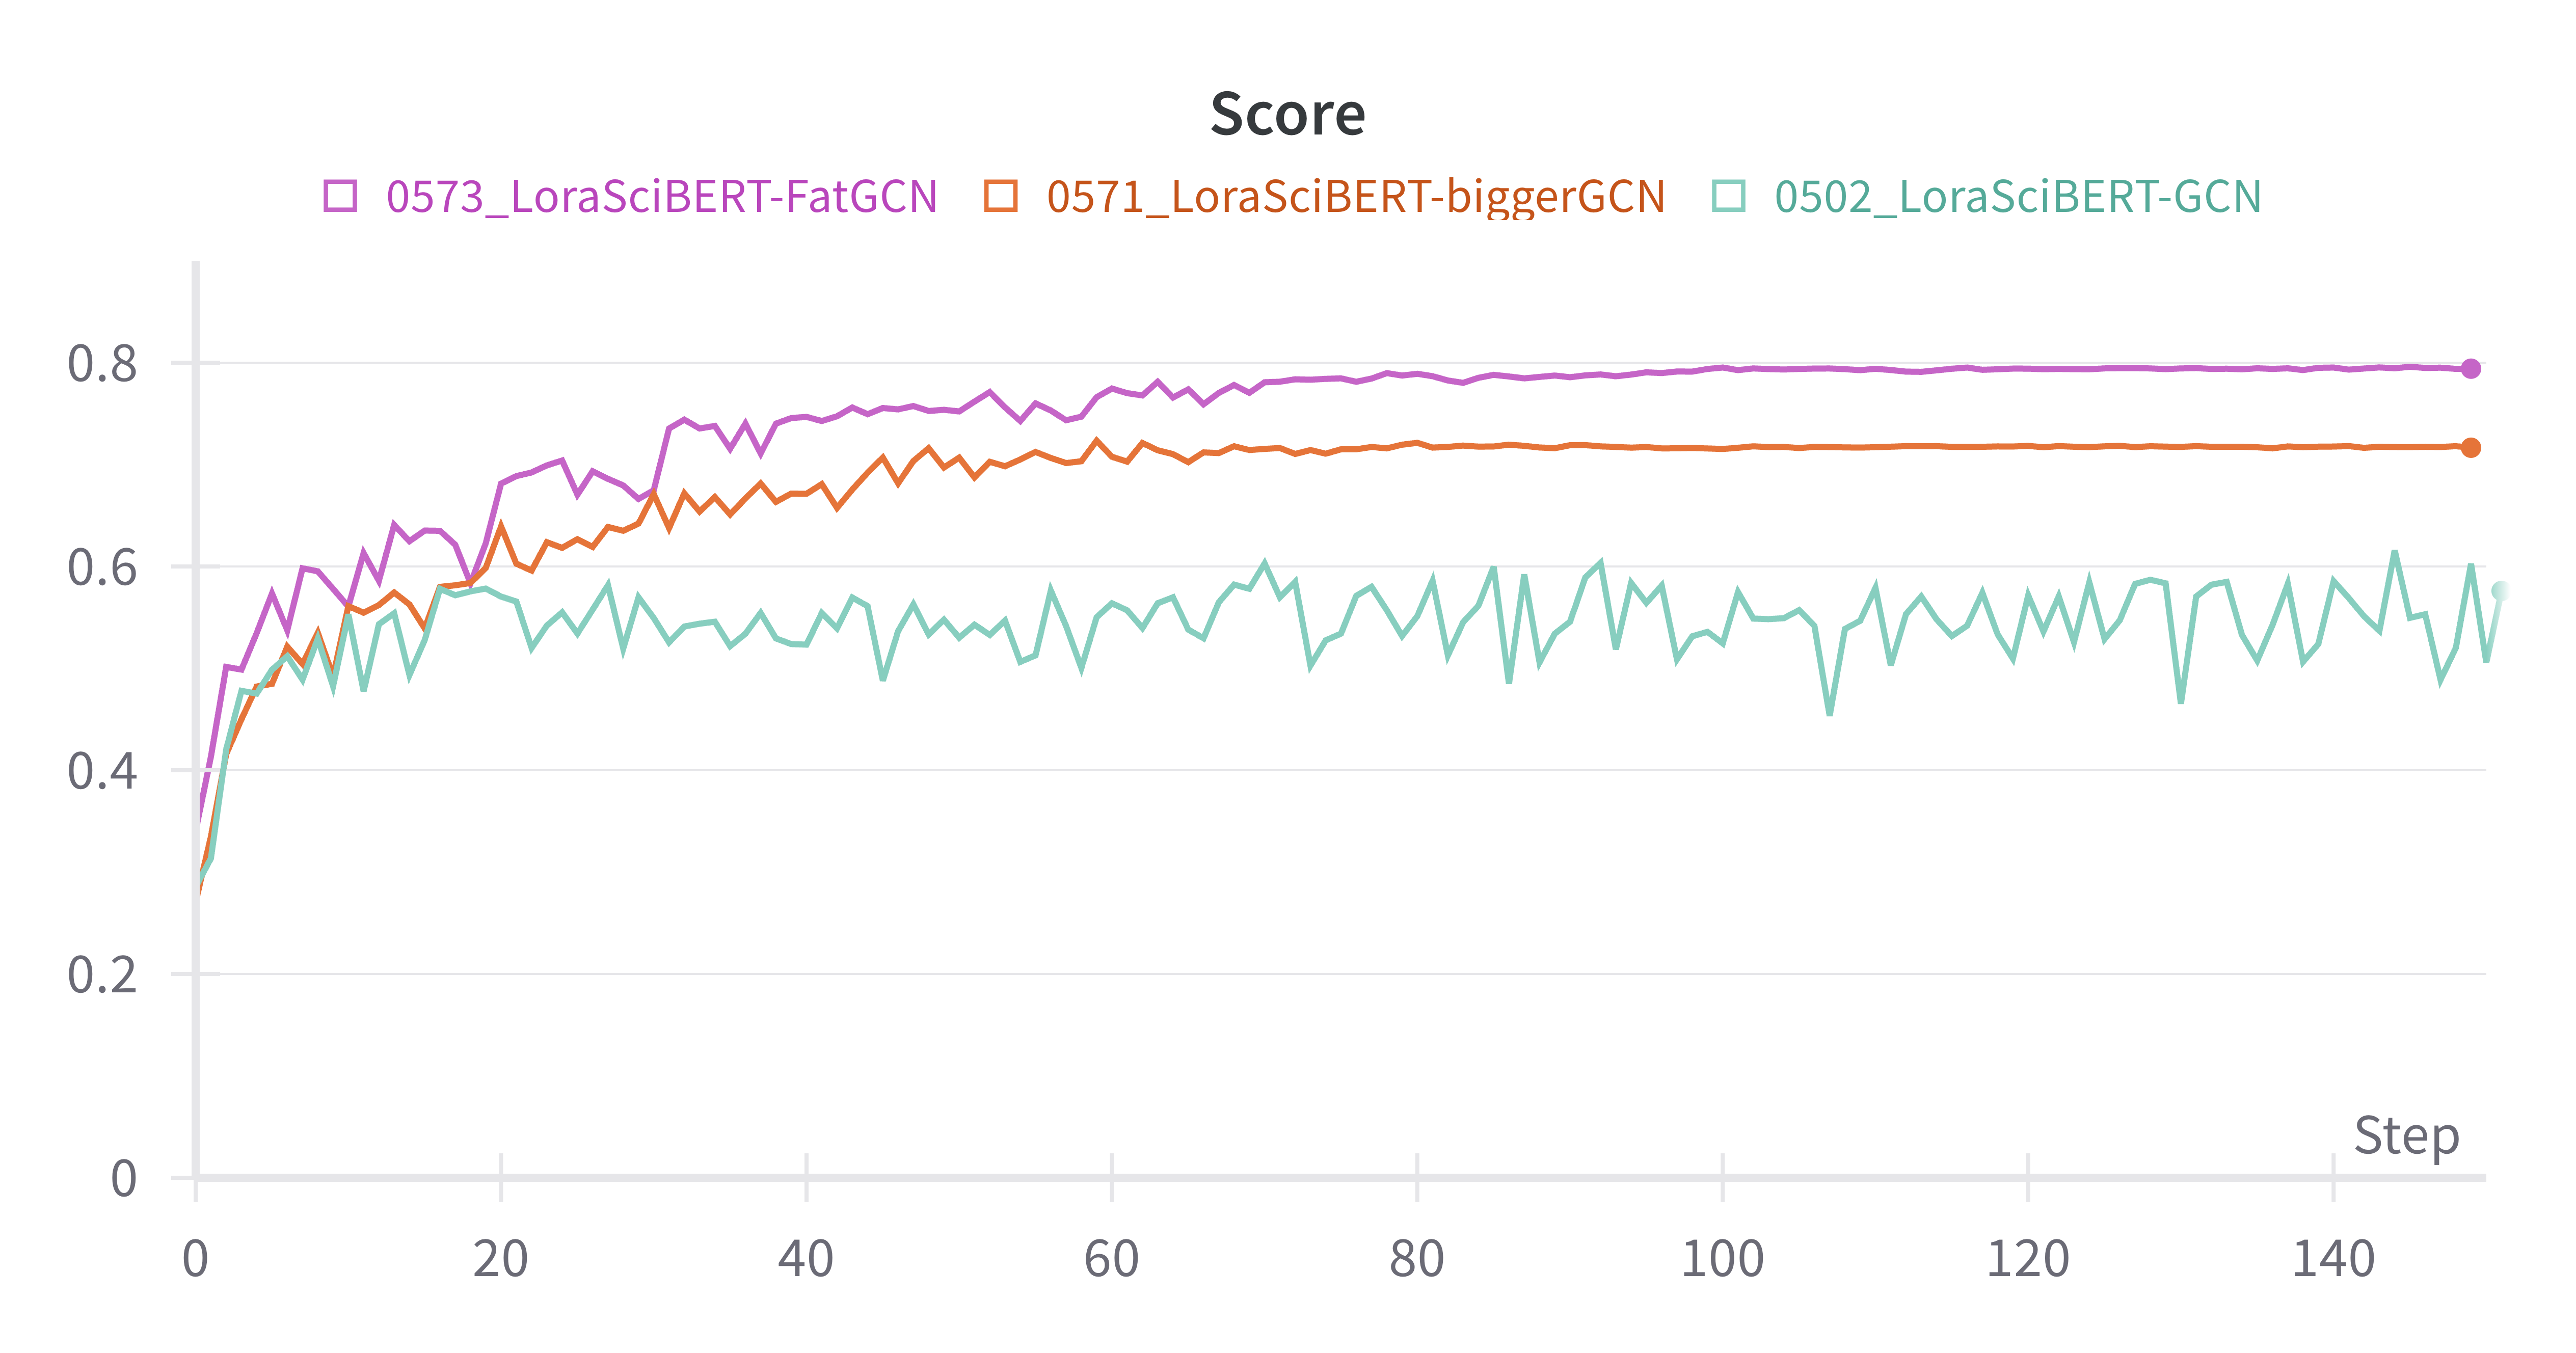
\includegraphics[width=0.3\textwidth]{figures/gcn.png}
\caption{LRAP scores for experiments 502, 571 and 573}
\label{gcn_fig}
\end{figure}

\subsection{Results for the best models trained with the contrastive loss}
\label{sec:best_old}

Out of all the experiments we led in the first part of our study with the initial contrastive loss provided with the baseline for this project, these 4 experiments are the ones that yielded the best LRAP scores. They were trained only using DistilBert in order to increase the batch size as much as possible and without LoRa which we did not feel helped us increase the batch size enough (complete architecture and parameters in Table \ref{tab:best_exp_old_loss}). All these experiments were performed using the same learning rate scheduler in "plateau" mode: initial learning rate of $3e-5$, "patience" of 8 epochs and decreasing factor of 0.8. We can see here that increasing the batch size can make up for a smaller GCN architecture and vice-versa and we obtained very similar results with all these experiments. Their scores are visible in Figure \ref{fig:old_best}.

\begin{table*}[!]
    \centering
    \begin{tabular}{|c|c|c|c|c|}
    \hline
    \textbf{Experiment ID} & \textbf{Model size} & \textbf{Batch size} & \textbf{GNN} & \textbf{LRAP} \\ \hline
    9008         & 67.9M & 164      & Bigger GCN 5 layers & 85.6\%      \\ \hline
     9009         &68.4M &  128      & Fat GCN 7 layers   & 85.9\%  \\ \hline
     9010         & 68.4M & 144      & Fat GCN 7 layers   & 86.1\%     \\ \hline
     9011        & 67.9M & 180      & Big GCN 5 layers  & 86.1\% \\ \hline

    \end{tabular}
    \caption{Successful experiments trained with the contrastive loss}
    \label{tab:best_exp_old_loss}
\end{table*}

\begin{figure}
\centering
\begin{minipage}{0.4\textwidth}
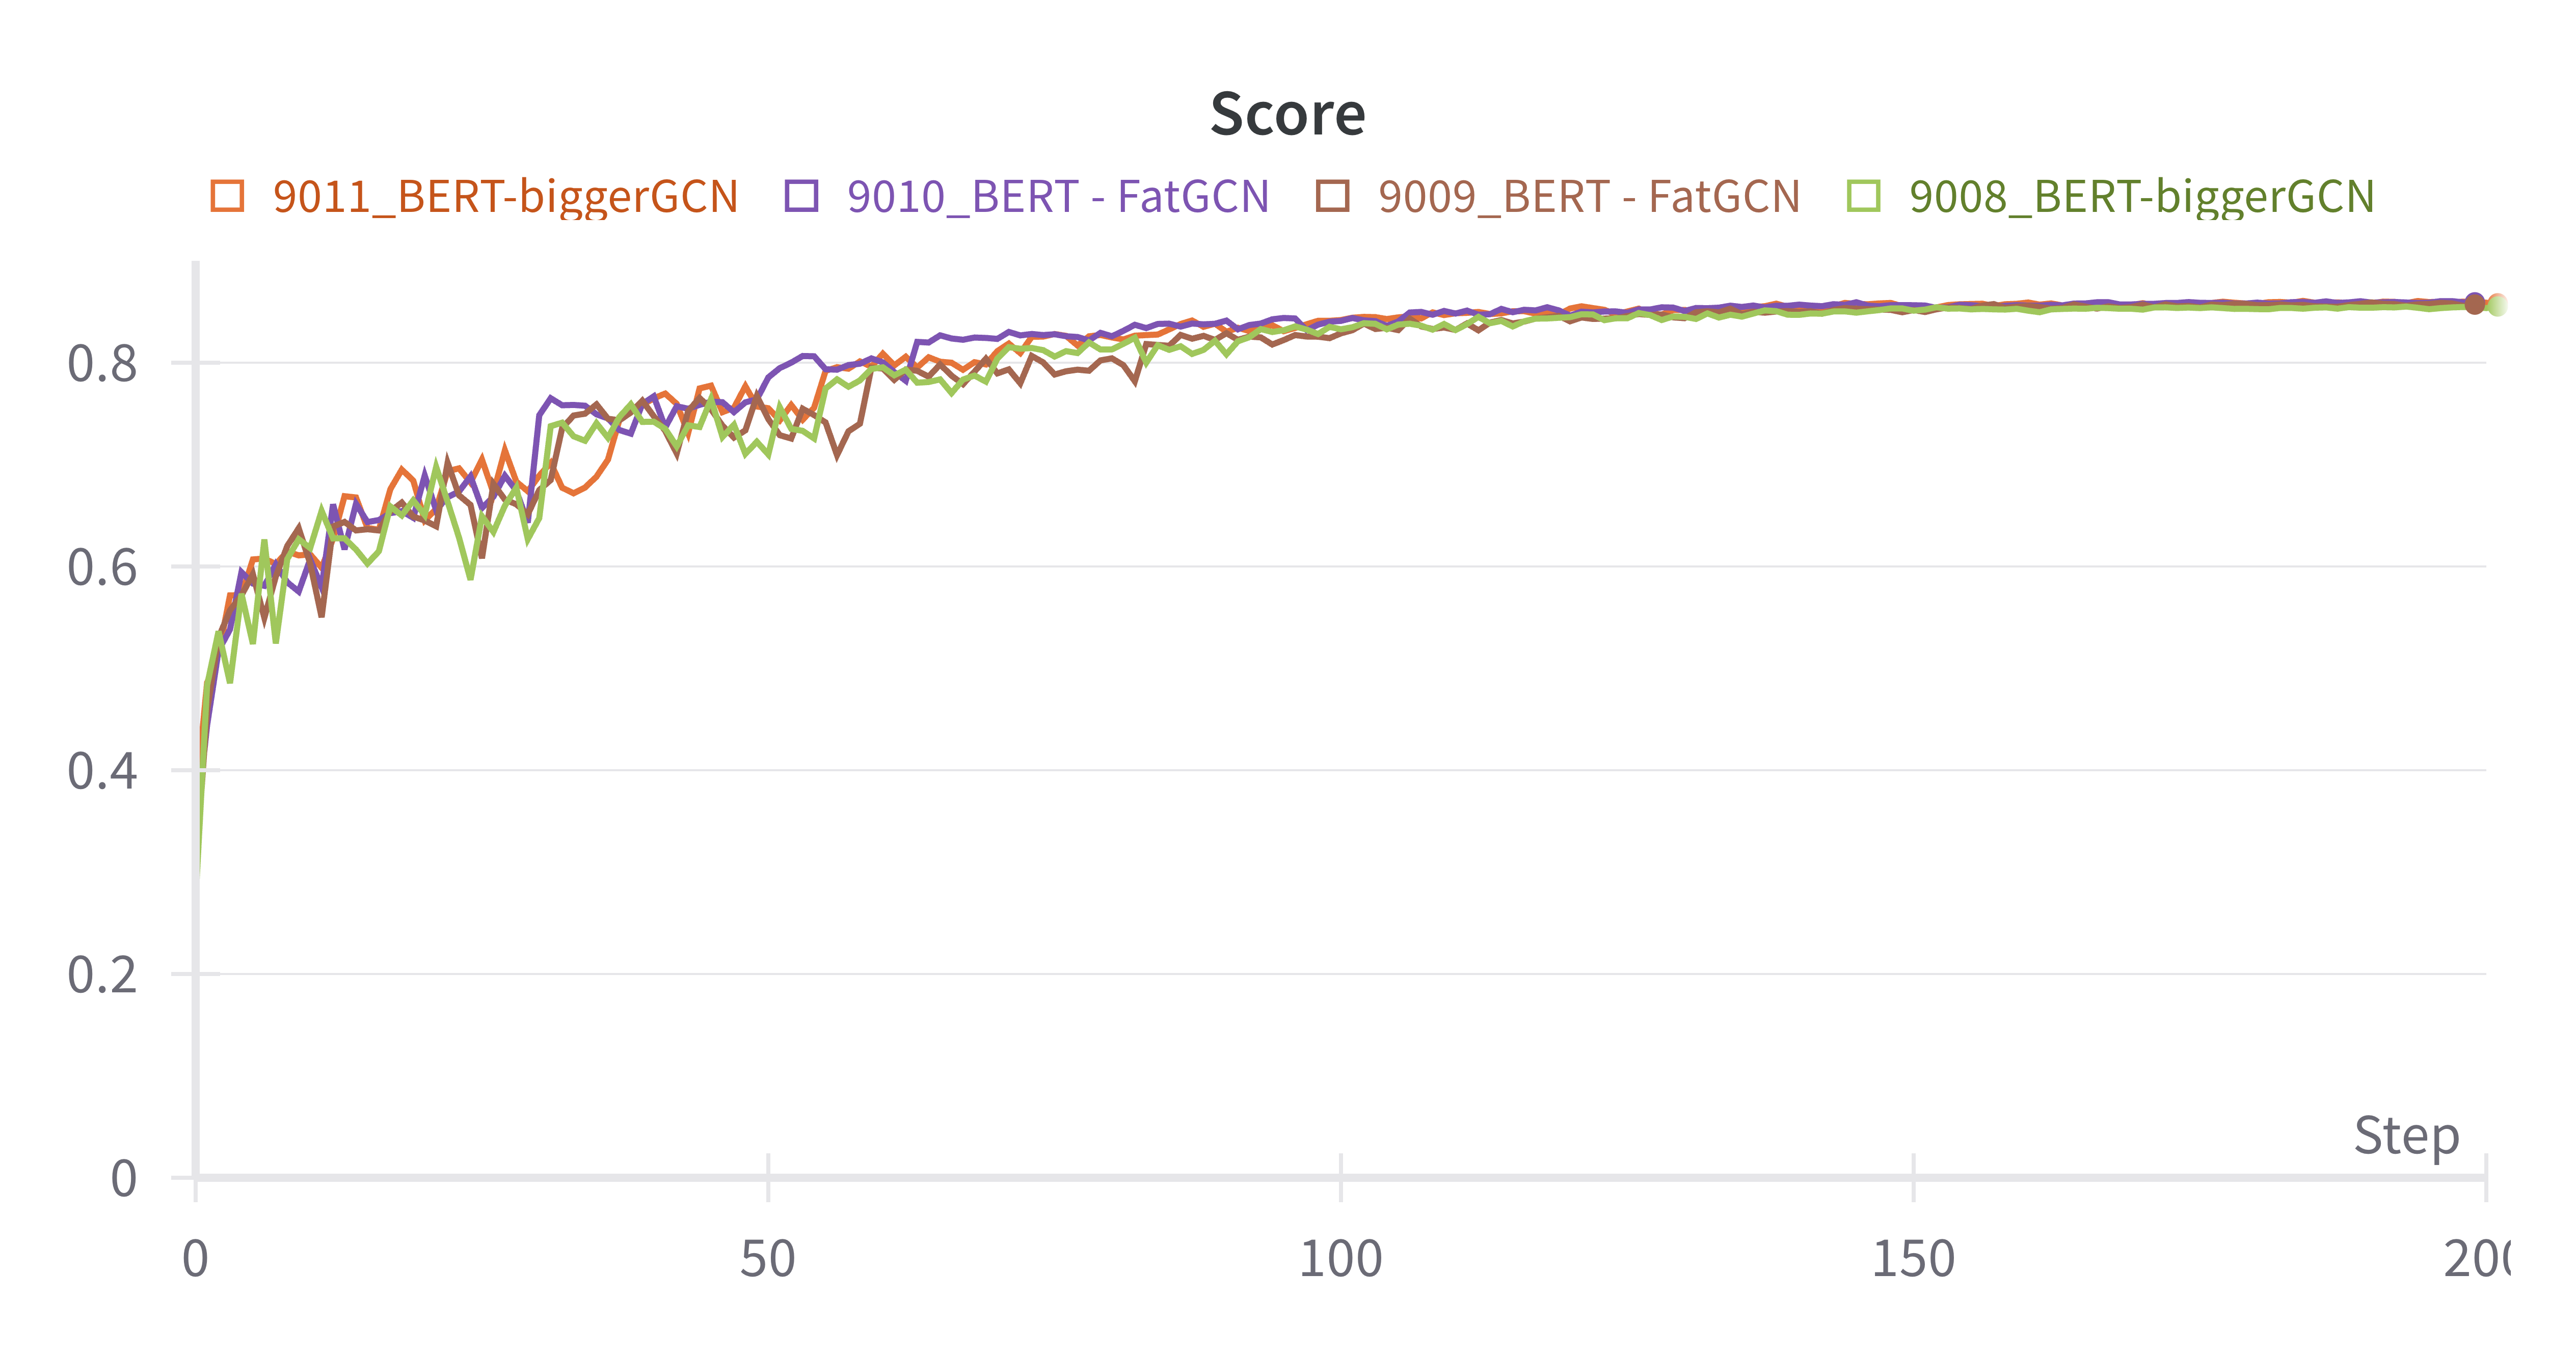
\includegraphics[width=\textwidth]{figures/9010_score.png}
\end{minipage}
\hfill
\begin{minipage}{0.4\textwidth}
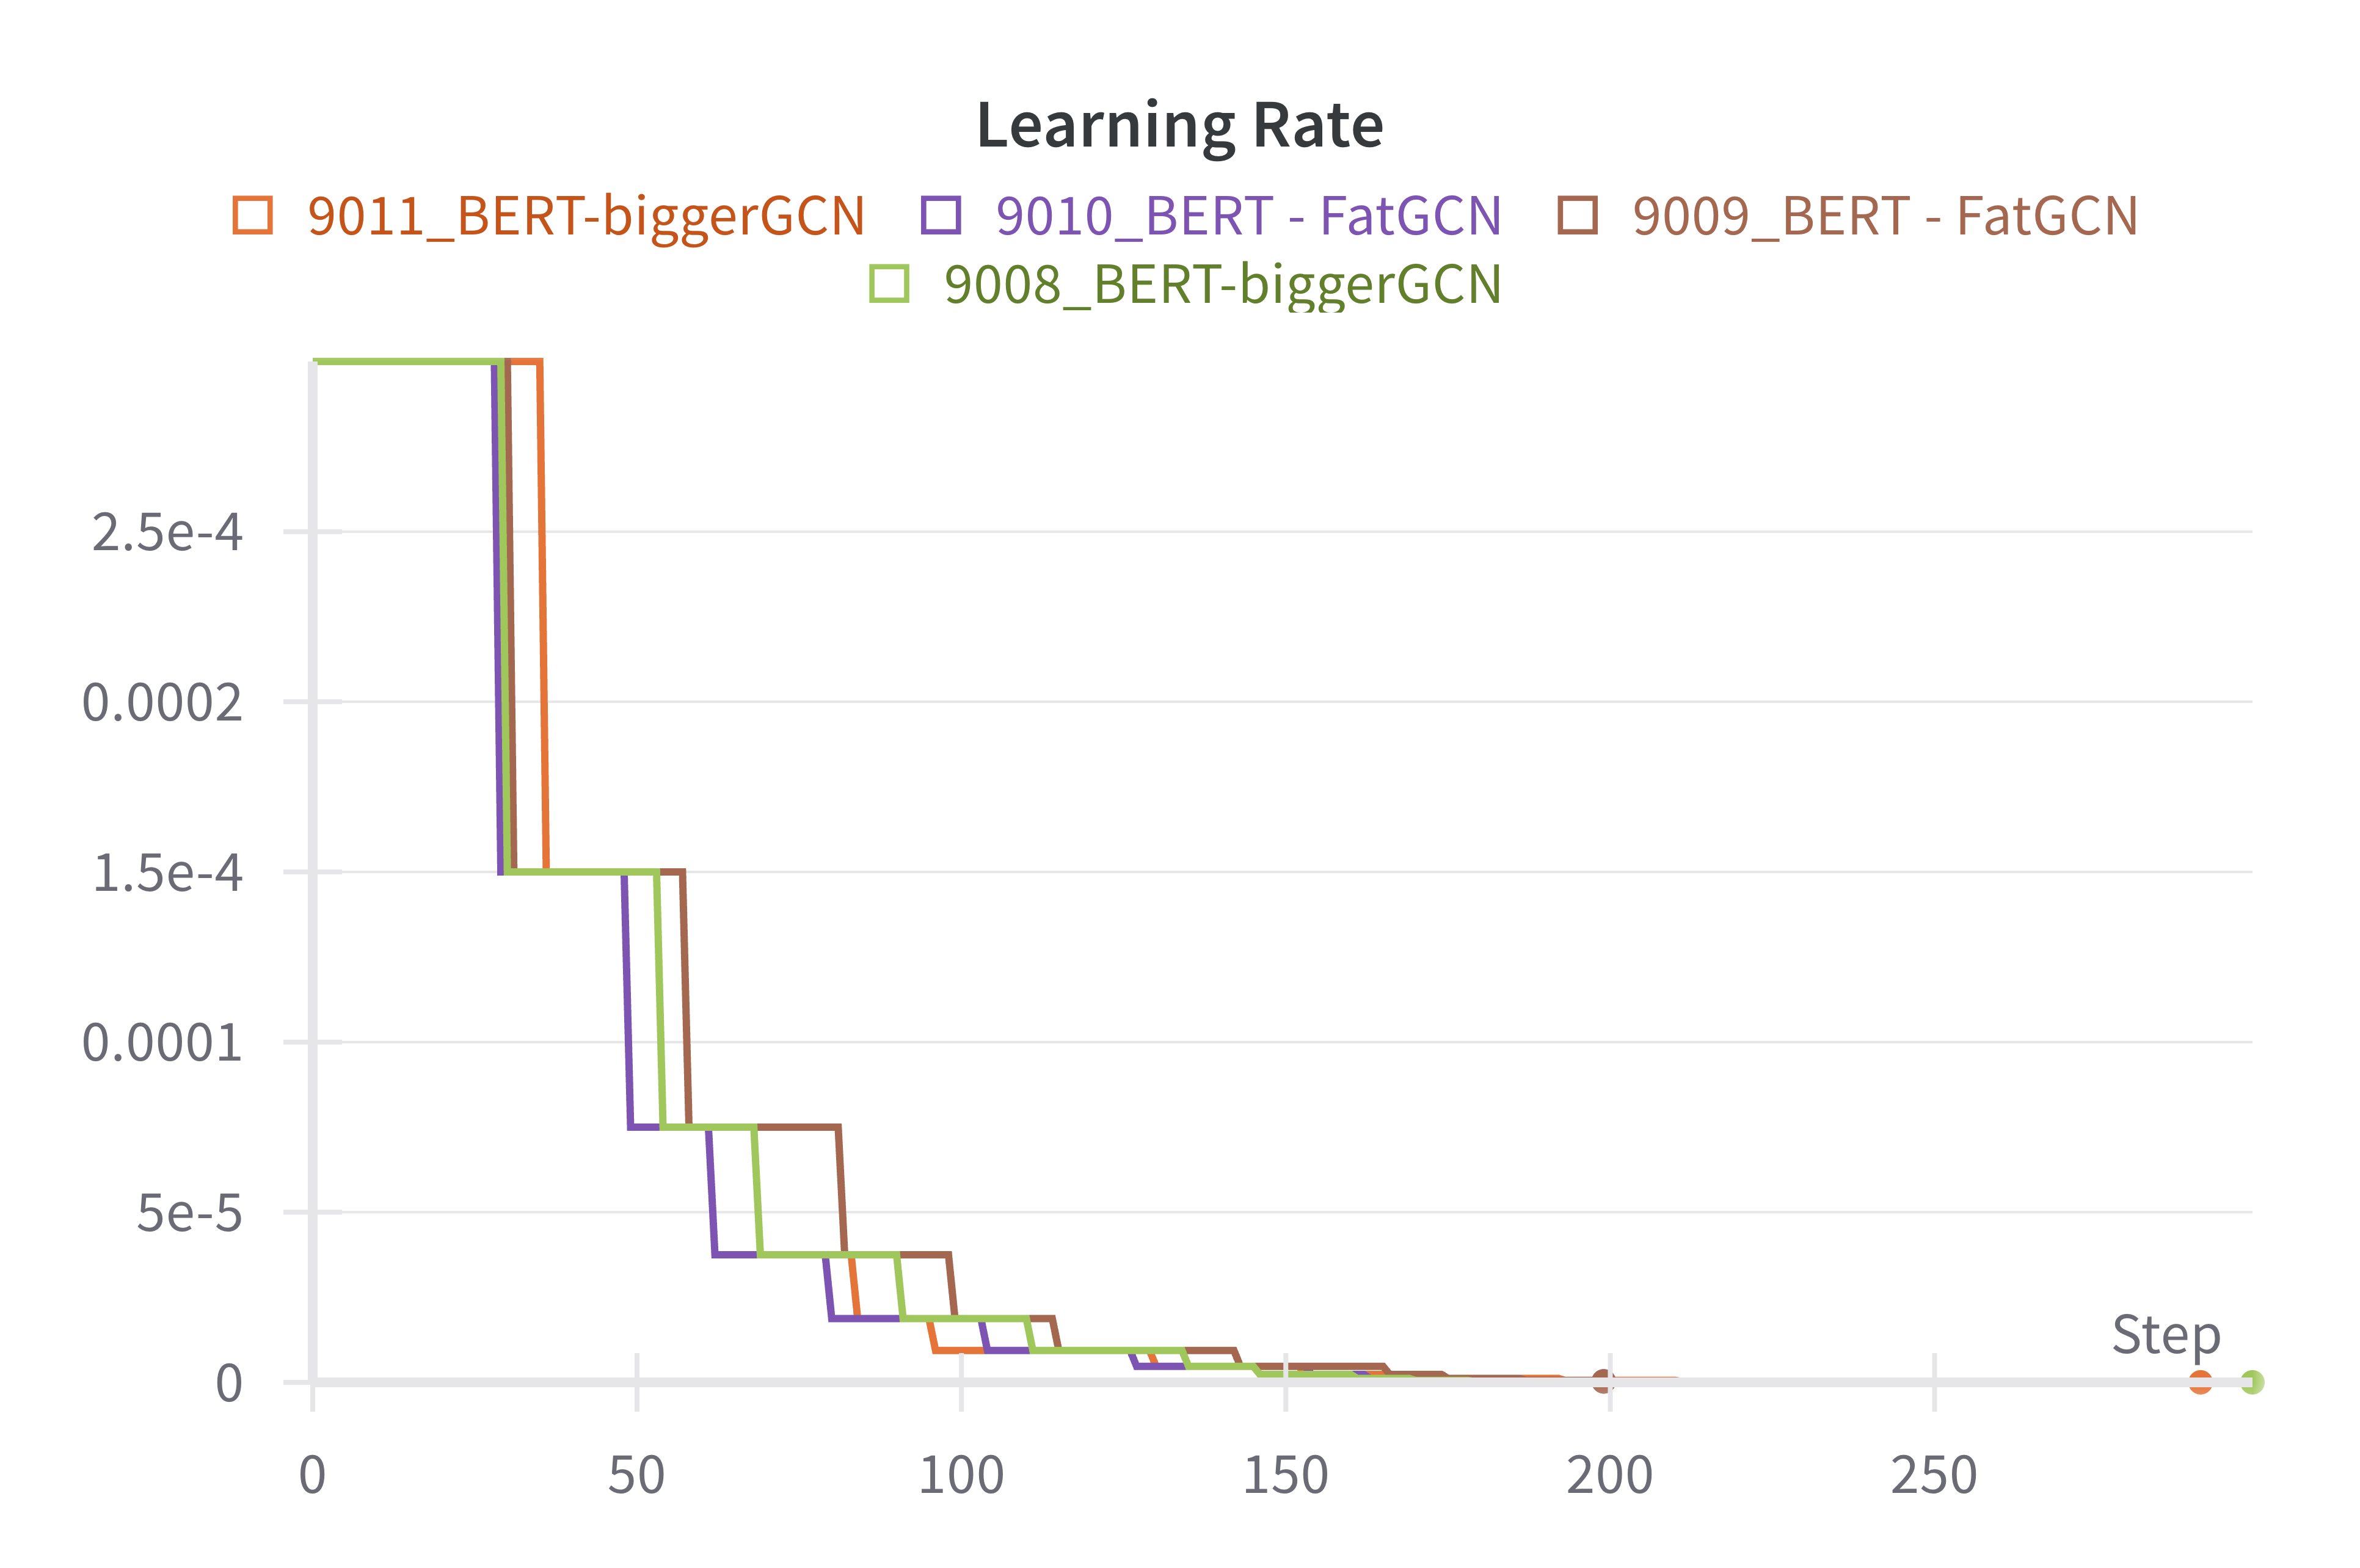
\includegraphics[width=\textwidth]{figures/W&B Chart 04_02_2024 10_34_42.png}   
\end{minipage}
\caption{Score for various successful experiments trained with the contrastive loss}
\label{fig:old_best}
\end{figure}

\subsection{Results for experiments trained with the binary contrastive loss}

\subsubsection{Baseline experiments}
\label{sec:baseline_new}

We trained the baseline experiments (BERT encoder and basic 3 layer GCN) with this new binary contrastive loss.Their detailed parameters can be found in Table \ref{tab:base_new_loss}. We used the learning rate 1e-4 proposed in \cite{text2mol}. We observe that the results (displayed on Figure \ref{baseline_fig}) are much higher than the previous best result on the baseline (experiment 68, LRAP score of 66\%).
\begin{table*}[!]
    \centering
    \begin{tabular}{|c|c|c|c|c|}
    \hline
    \textbf{Experiment ID} & \textbf{Model size} & \textbf{Batch size} &\textbf{Loss} & \textbf{LRAP} \\ \hline
    18         & 67.0M & 32      & Binary contrastive  & 71.5\%      \\ \hline
     19       & 67.0M  &  64      & Binary contrastive  & 79.9\%  \\ \hline
     20        & 67.0M &  128      & Binary contrastive  & 77\%     \\ \hline
     68     &67.0M   &  128     & Contrastive  & 66.7\% \\ \hline

    \end{tabular}
    \caption{Baseline experiments with different training losses}
    \label{tab:base_new_loss}
\end{table*}

\begin{figure}
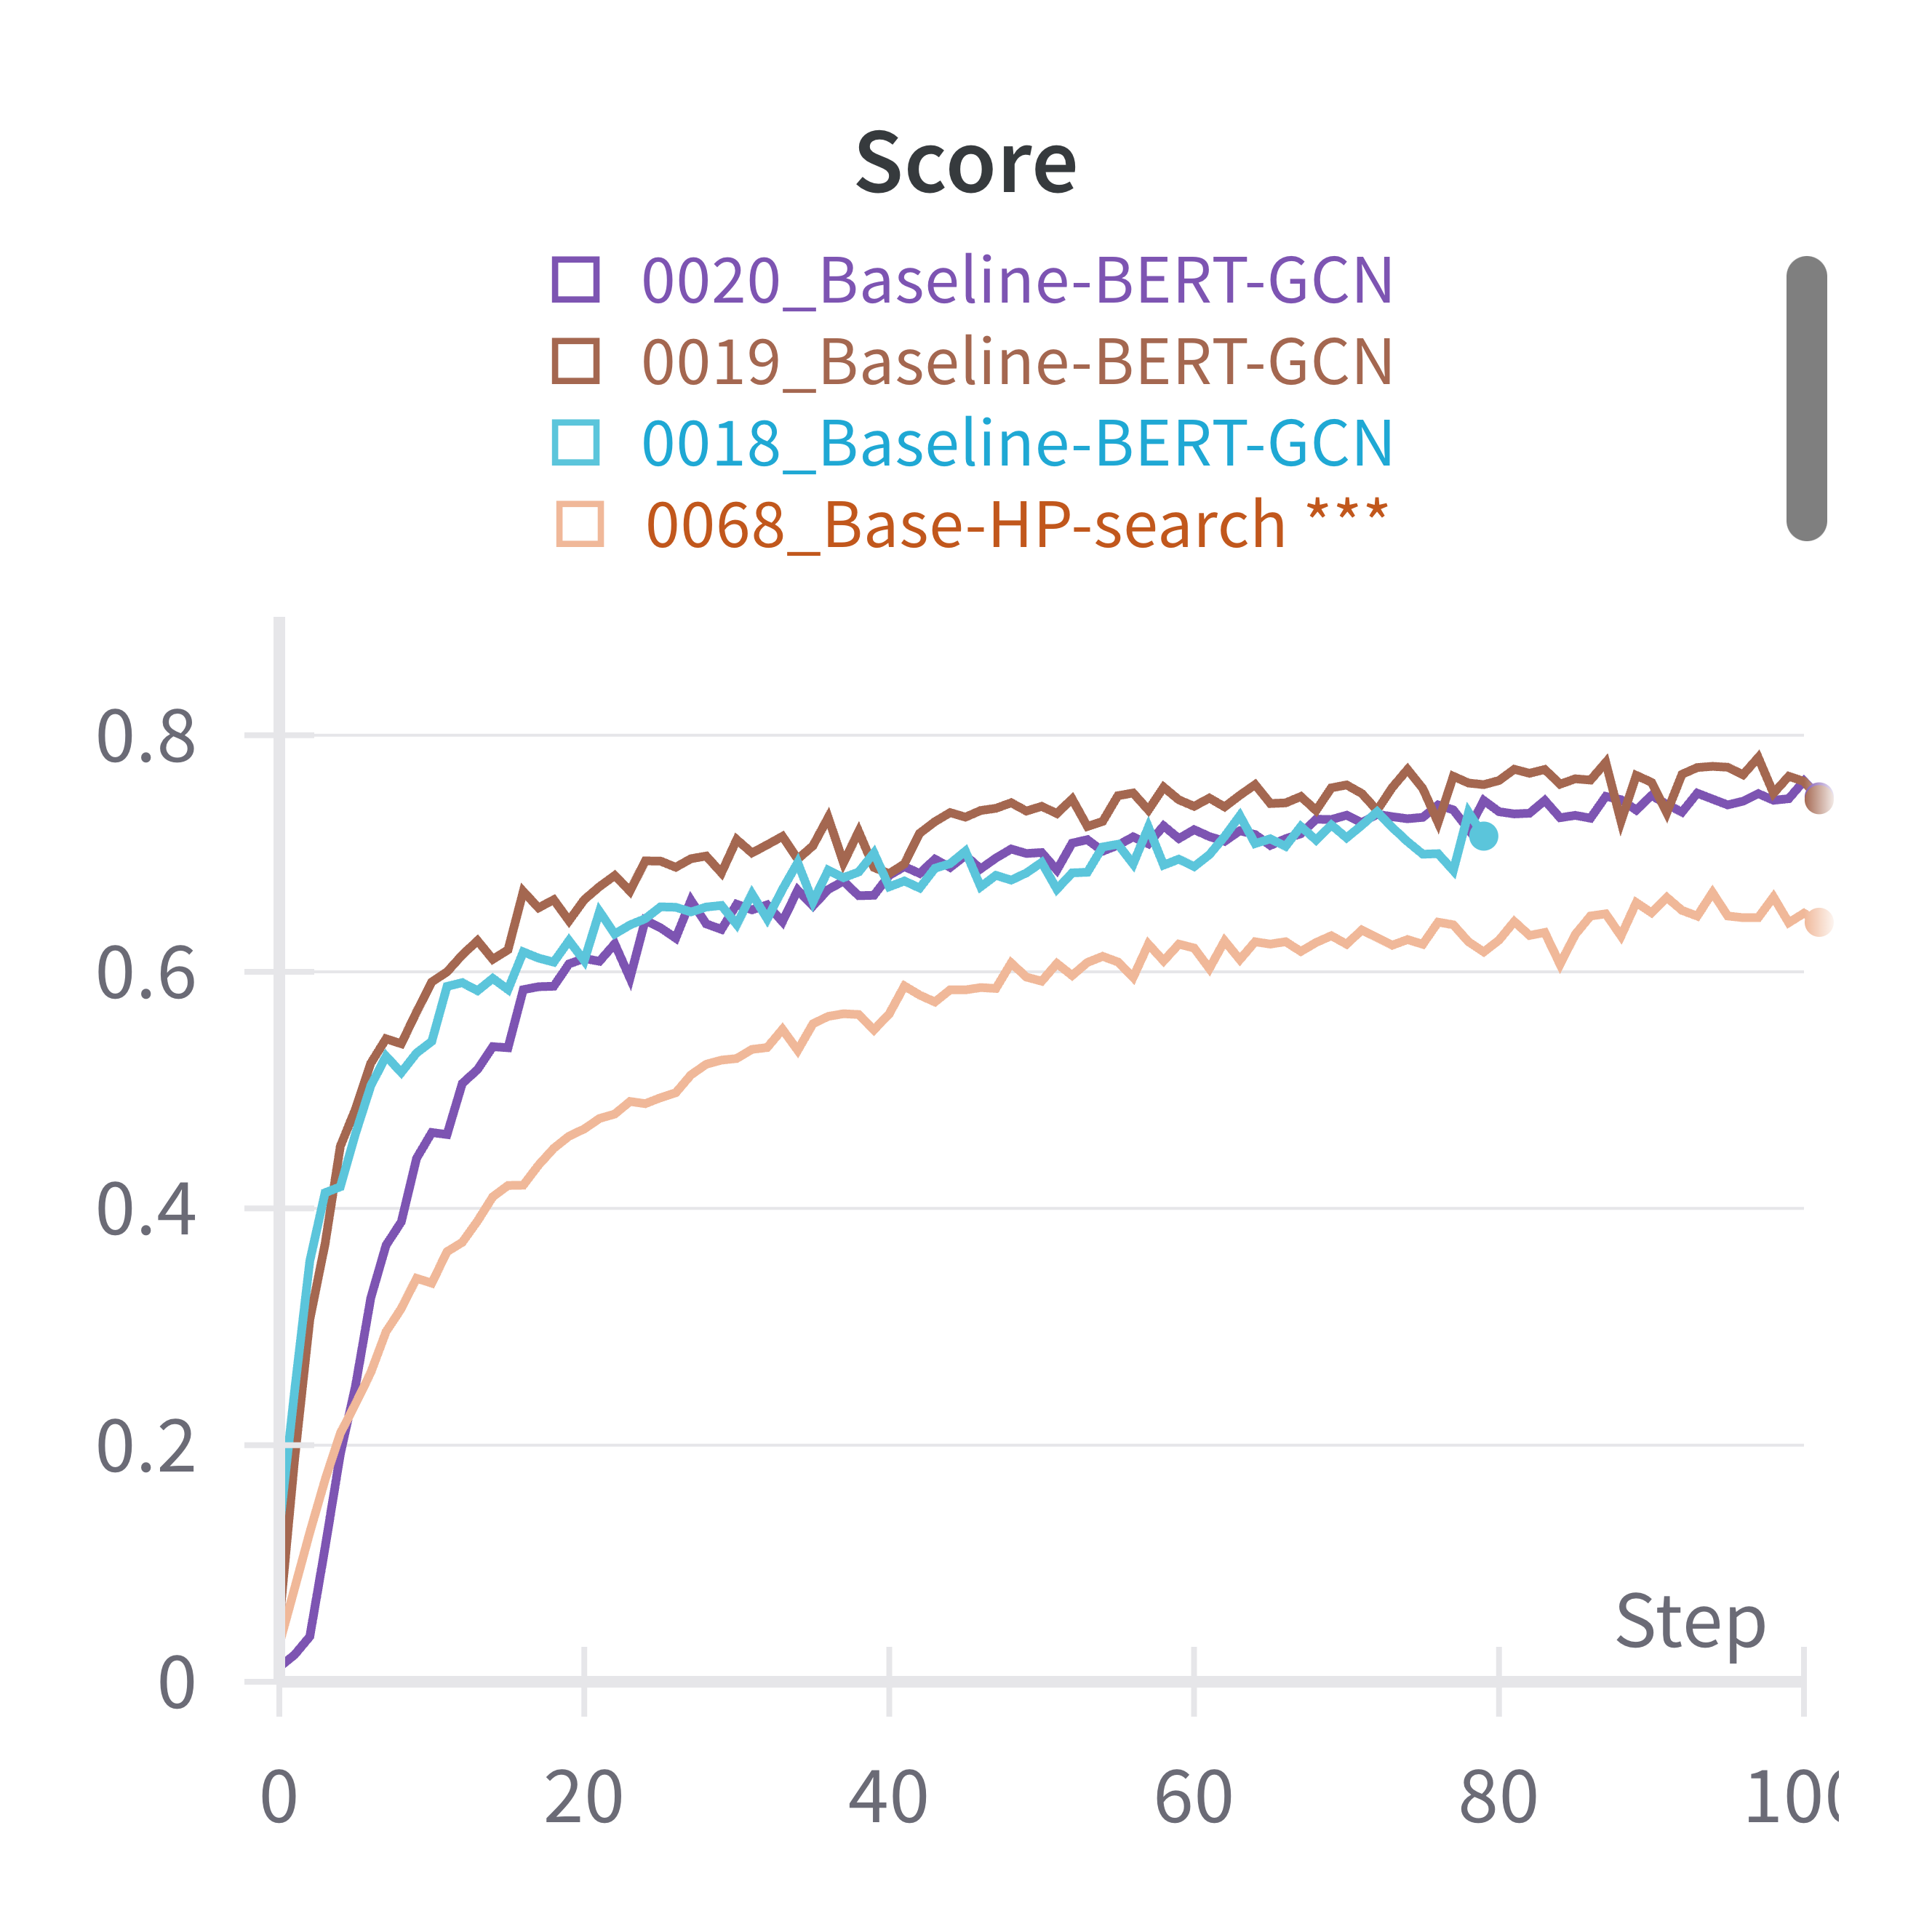
\includegraphics[width=0.3\textwidth]{figures/baseline.png}
\caption{LRAP score for baseline experiments}
\label{baseline_fig}
\end{figure}

\subsubsection{Other successful experiments}
\label{sec:best_new}
In order to get other models with high scores, we reproduced models with an architecture similar to those of experiments 9008-9011 and trained them with the binary contrastive loss. These architectures are presented in further detail in Table \ref{tab:best_new_loss}.Thanks to this loss, we were able to achieve similar results with smaller batches during training. We retained the learning scheduler (initial $lr=1e-4$) and DistilBERT encoder and played with the graph and the batch sizes to obtain high performances. The scores of all these experiments are displayed on Figure \ref{fig:best_new_loss}. 

\begin{table*}[!]
    \centering
    \begin{tabular}{|c|c|c|c|c|}
    \hline
    \textbf{Experiment ID} & \textbf{Model size} & \textbf{Batch size} &\textbf{GNN} & \textbf{LRAP} \\ \hline
    9070         & 67.9M & 128      & Bigger GCN 5 layers  & 83.6\%      \\ \hline
     9072      & 67.0M  &  128      & Base GCN 3 layers  & 79.9\%  \\ \hline
     9073        & 67.9M &  64      & Bigger GCN 5 layers  & 83.0\%     \\ \hline
     9075     &68.4M   &  64     & Fat GCN 7 layers  & 86.1\% \\ \hline
      9077     & 68.4M  &  92     & Fat GCN 7 layers  & 86.3\% \\ \hline
    \end{tabular}
    \caption{Experiments with binary contrastive training loss}
    \label{tab:best_new_loss}
\end{table*}

\begin{figure}
\centering
\begin{minipage}{0.4\textwidth}
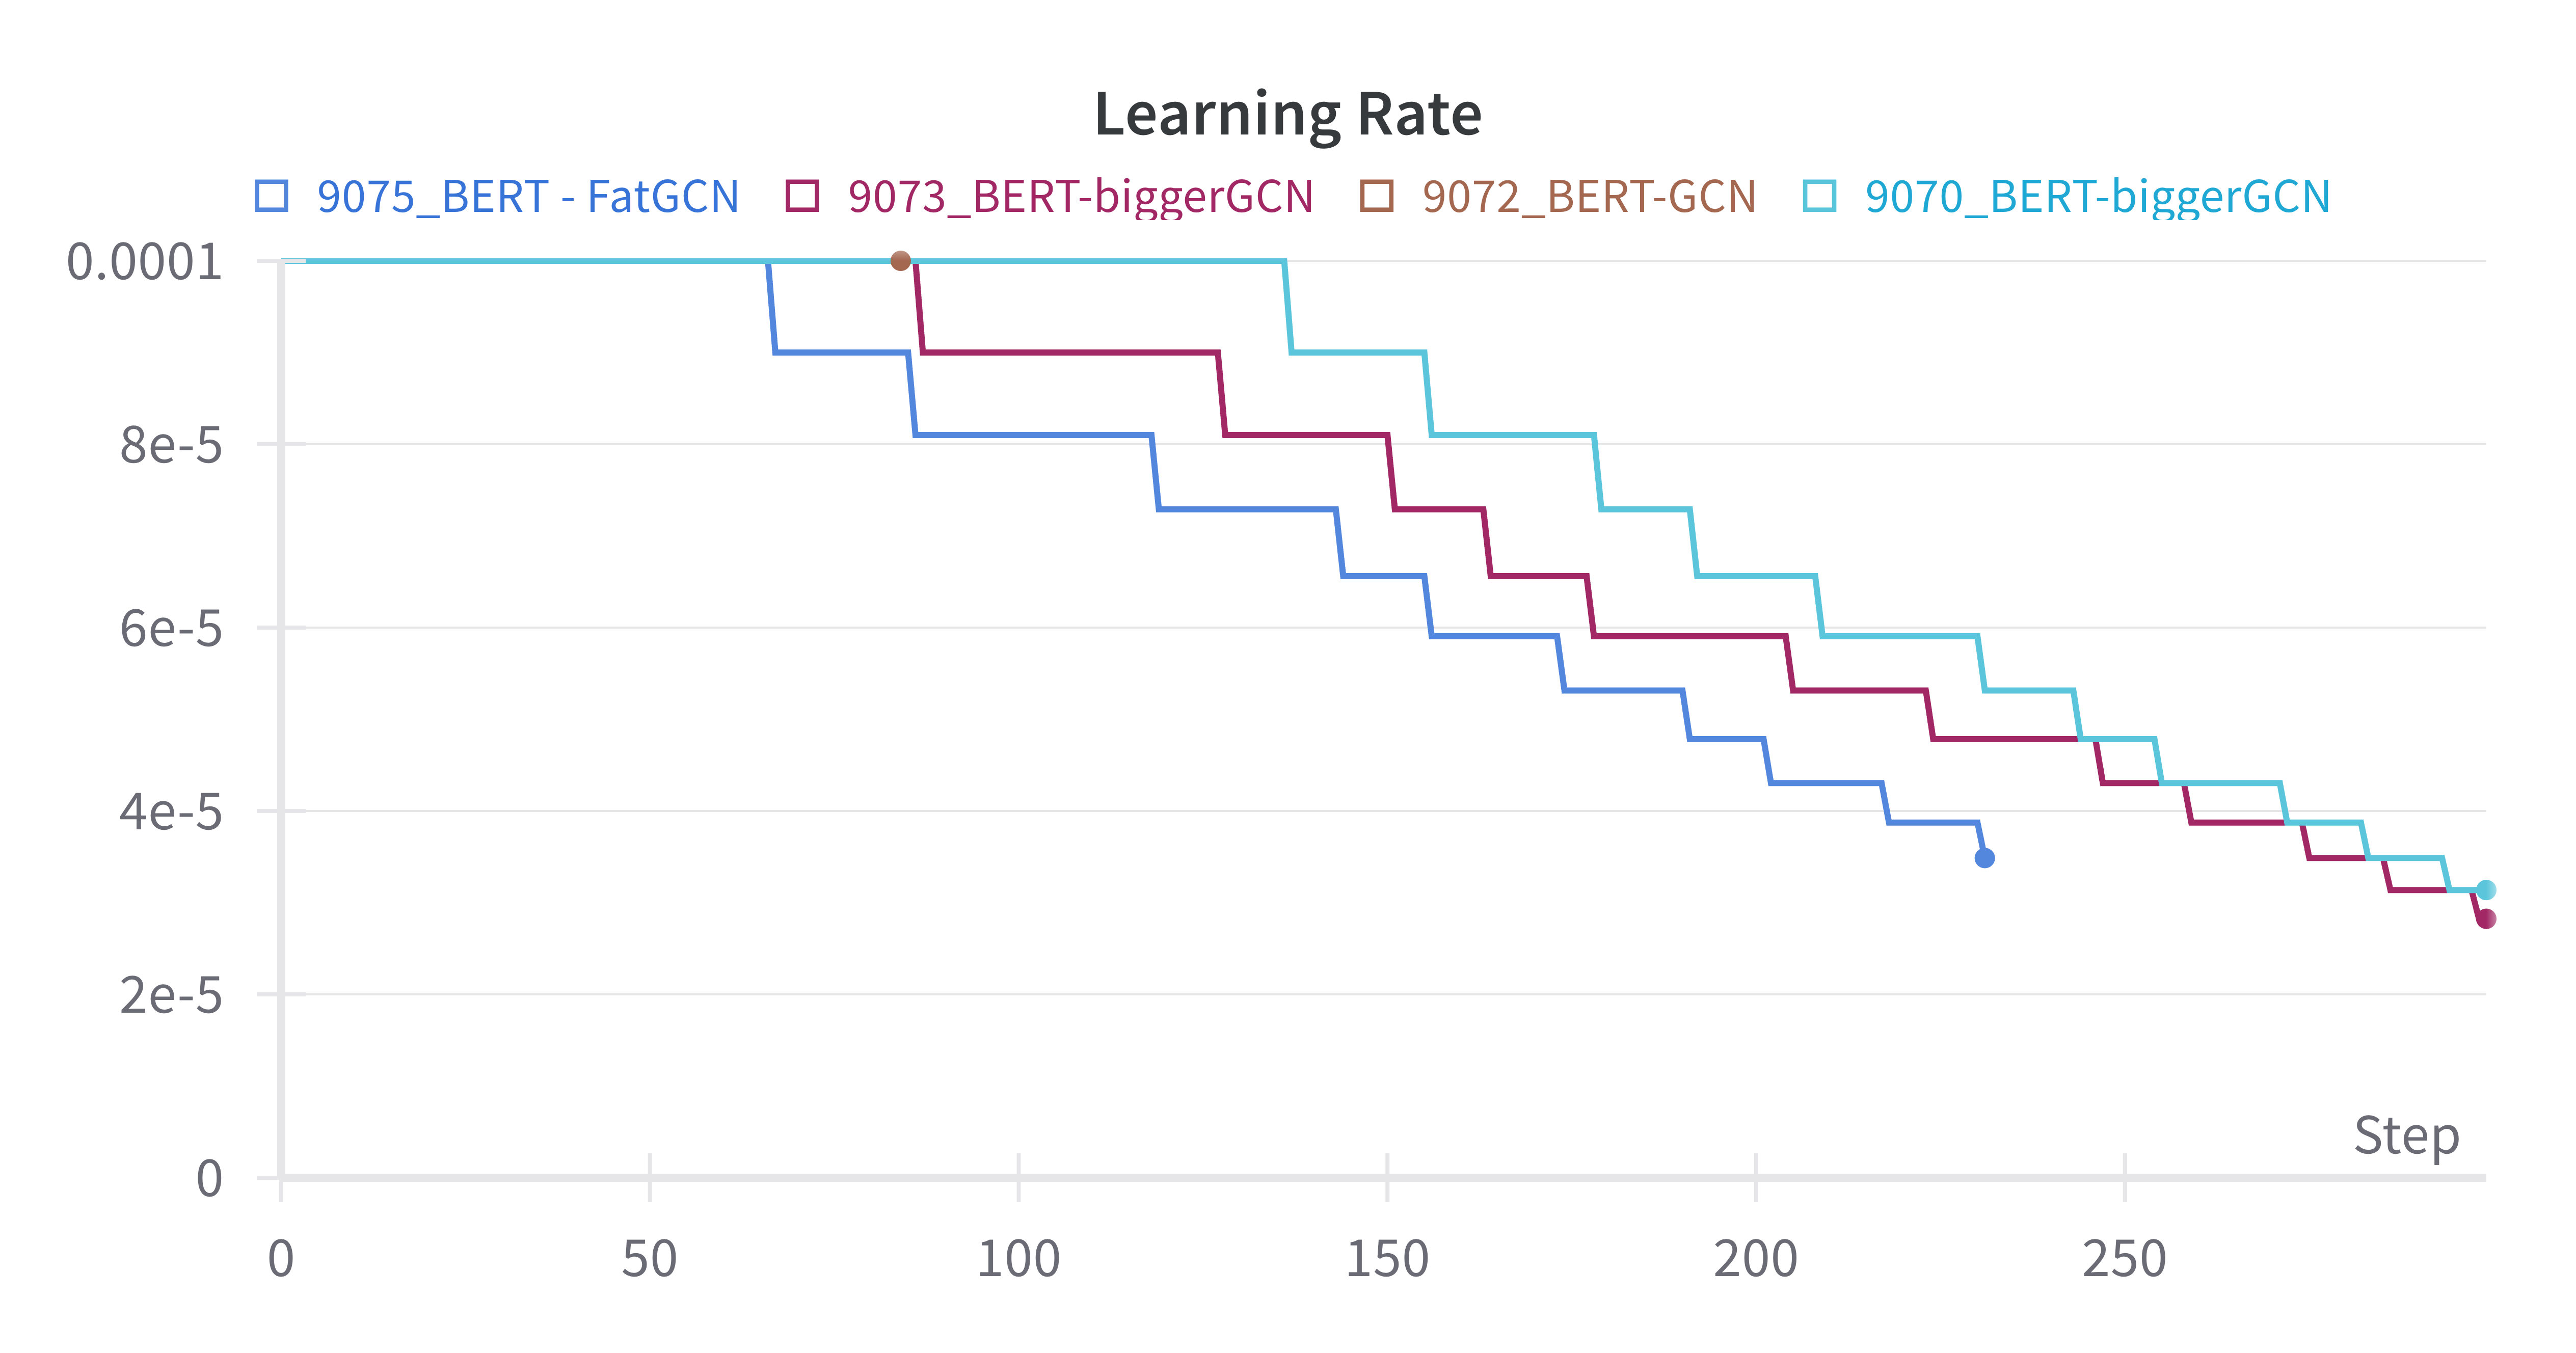
\includegraphics[width=\textwidth]{figures/9070_lr.png}
\end{minipage}
\hfill
\begin{minipage}{0.4\textwidth}
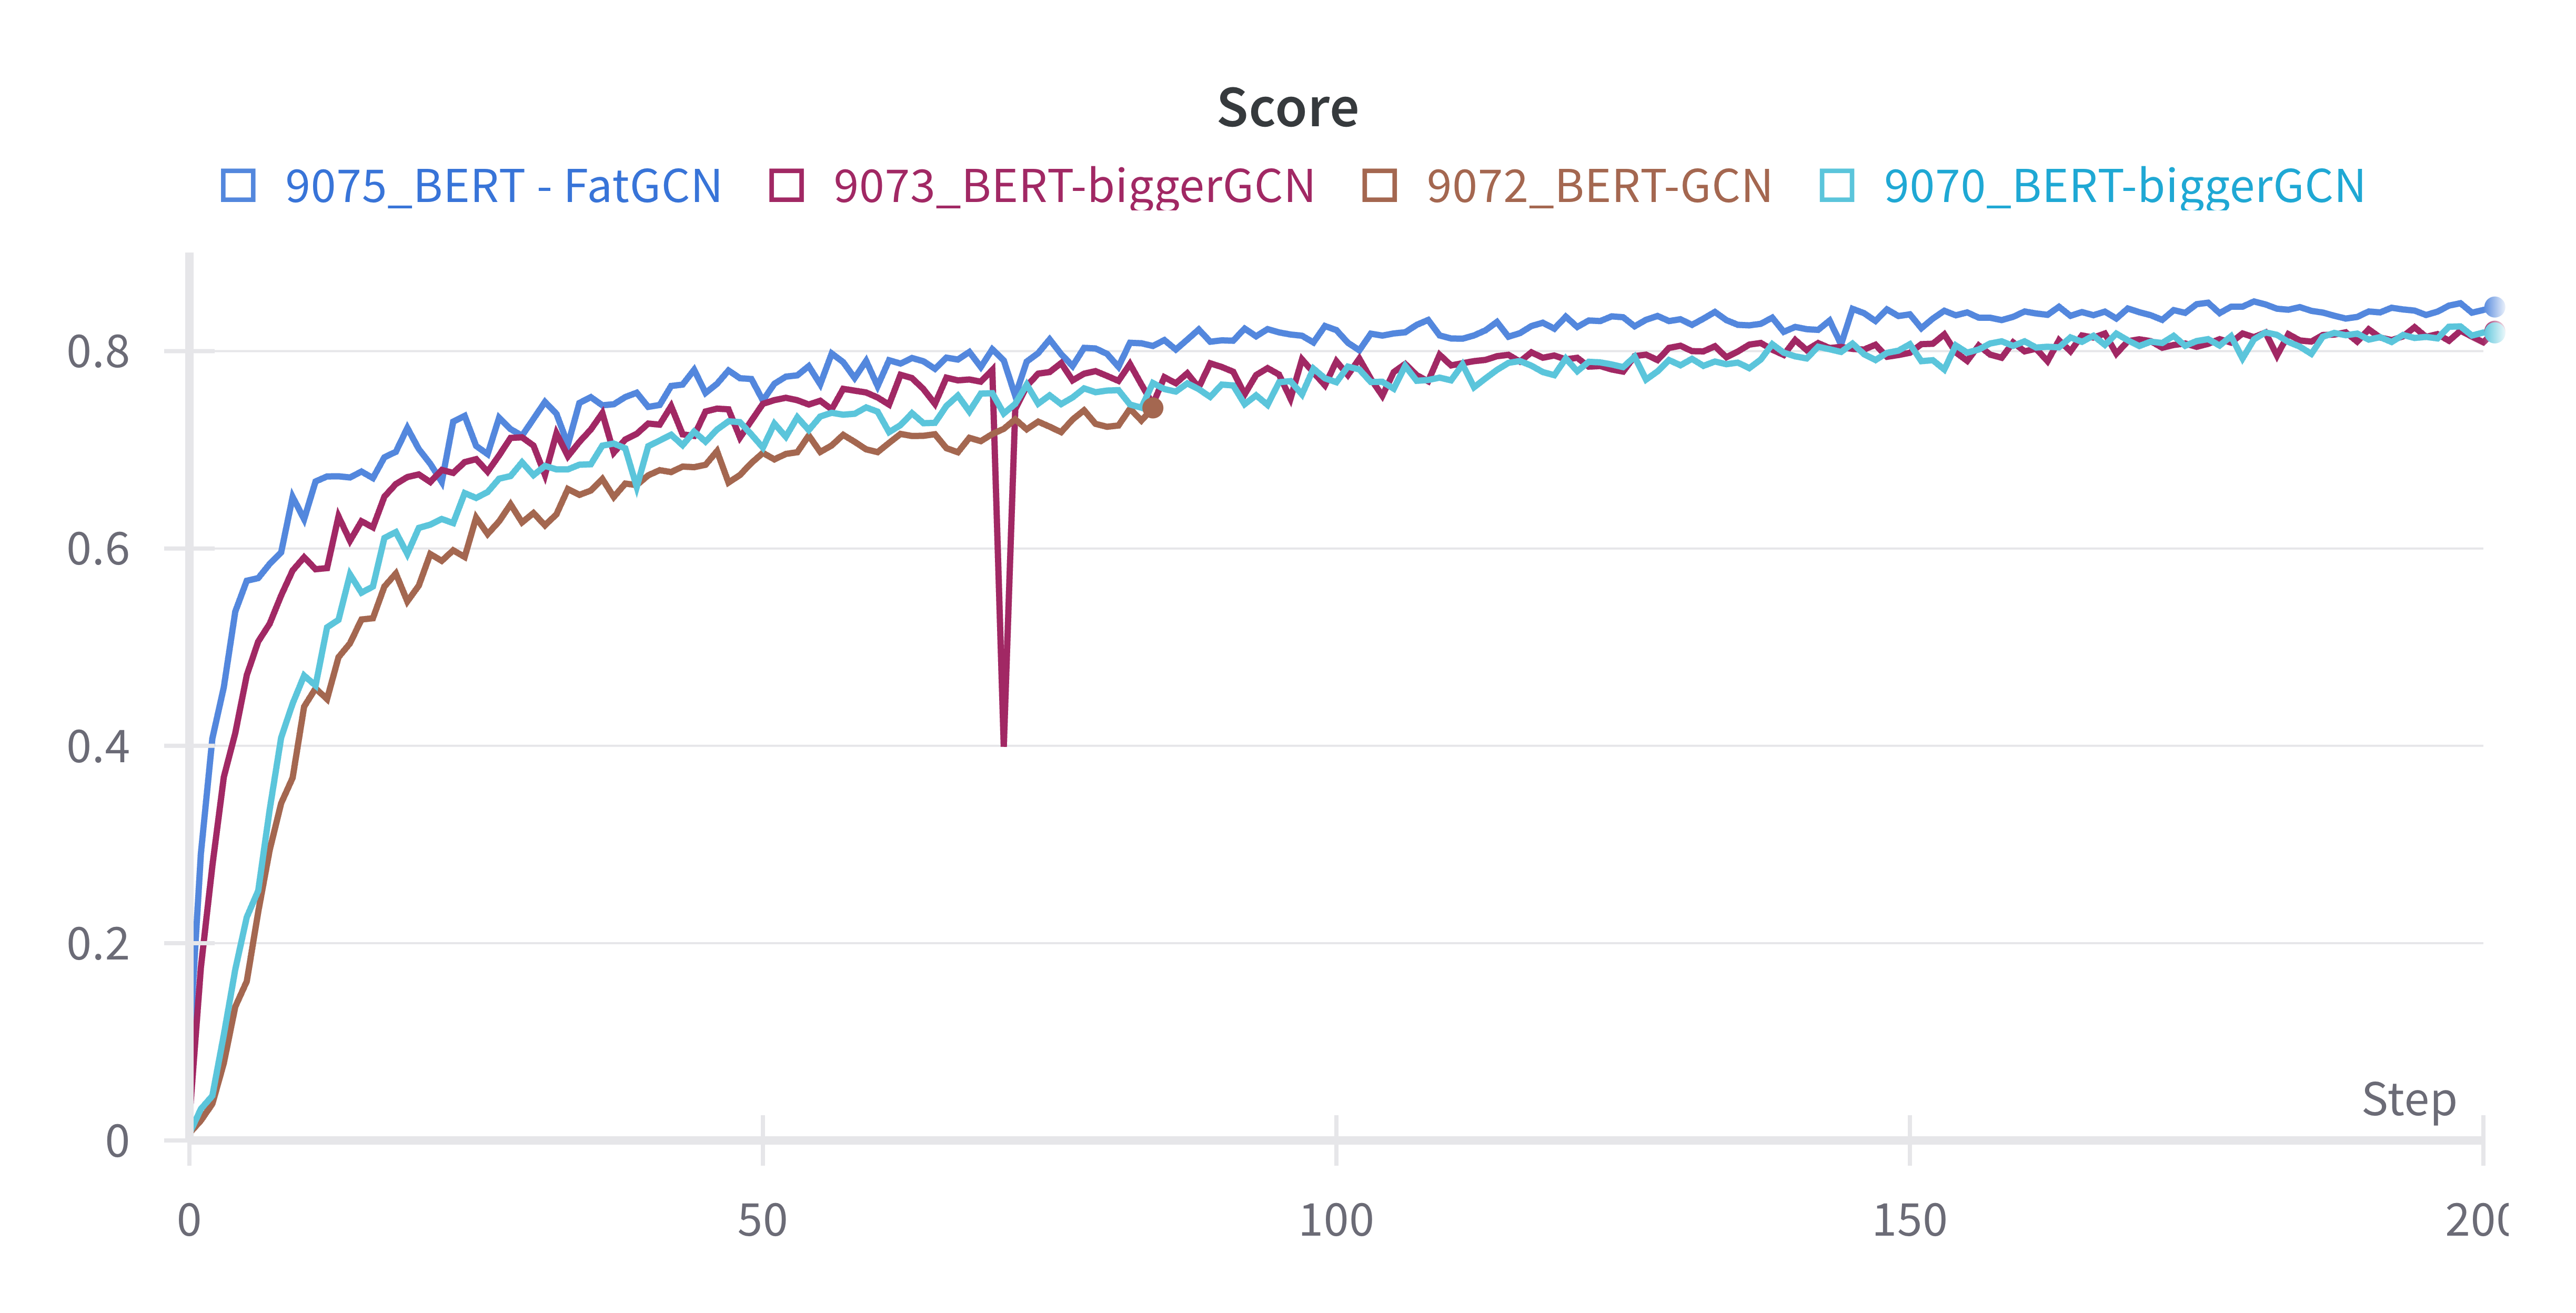
\includegraphics[width=\textwidth]{figures/9070_score.png}   
\end{minipage}
\caption{Score and learning rate for the best experiments with various GCN and batch sizes trained with the binary contrastive loss}
\label{fig:best_new_loss}
\end{figure}

\subsection*{Freezing the LLM, training a large GCN from scratch}
\label{sec:frozen}
We reused the trained model 573 which we already presented (Lora Scibert model trained with a batch size of 64, a learning rate scheduler and the 'Fat GCN' architecture) in experiment 611. We froze the trained LLM obtained via 573 and trained 611 with a bigger batch size. The details about these experiments can be found in Table \ref{tab:frozen_573} and their respective scores are displayed on Figure \ref{fig:611}. This technique enabled us to improve the LRAP score of 80\%  we had already obtained when training experiment 573. 
\begin{table*}[!]
    \centering
    \begin{tabular}{|c|c|c|c|c|}
    \hline
    \textbf{Experiment ID} & \textbf{Model size} & \textbf{Batch size} &\textbf{GNN} & \textbf{LRAP} \\ \hline
    573         & 3.4M & 64    & Fat GCN 7 layers  & 79.6\%      \\ \hline
     611 & 2.4 & 192 & Fat GCN 7 layers & 86.7%\ \\ \hline
    \end{tabular}
    \caption{Fully trained experiment and experiment with the frozen LLM and GCN trained from scratch}
    \label{tab:frozen_573}
\end{table*}

\begin{figure}
\centering
\begin{minipage}{0.4\textwidth}
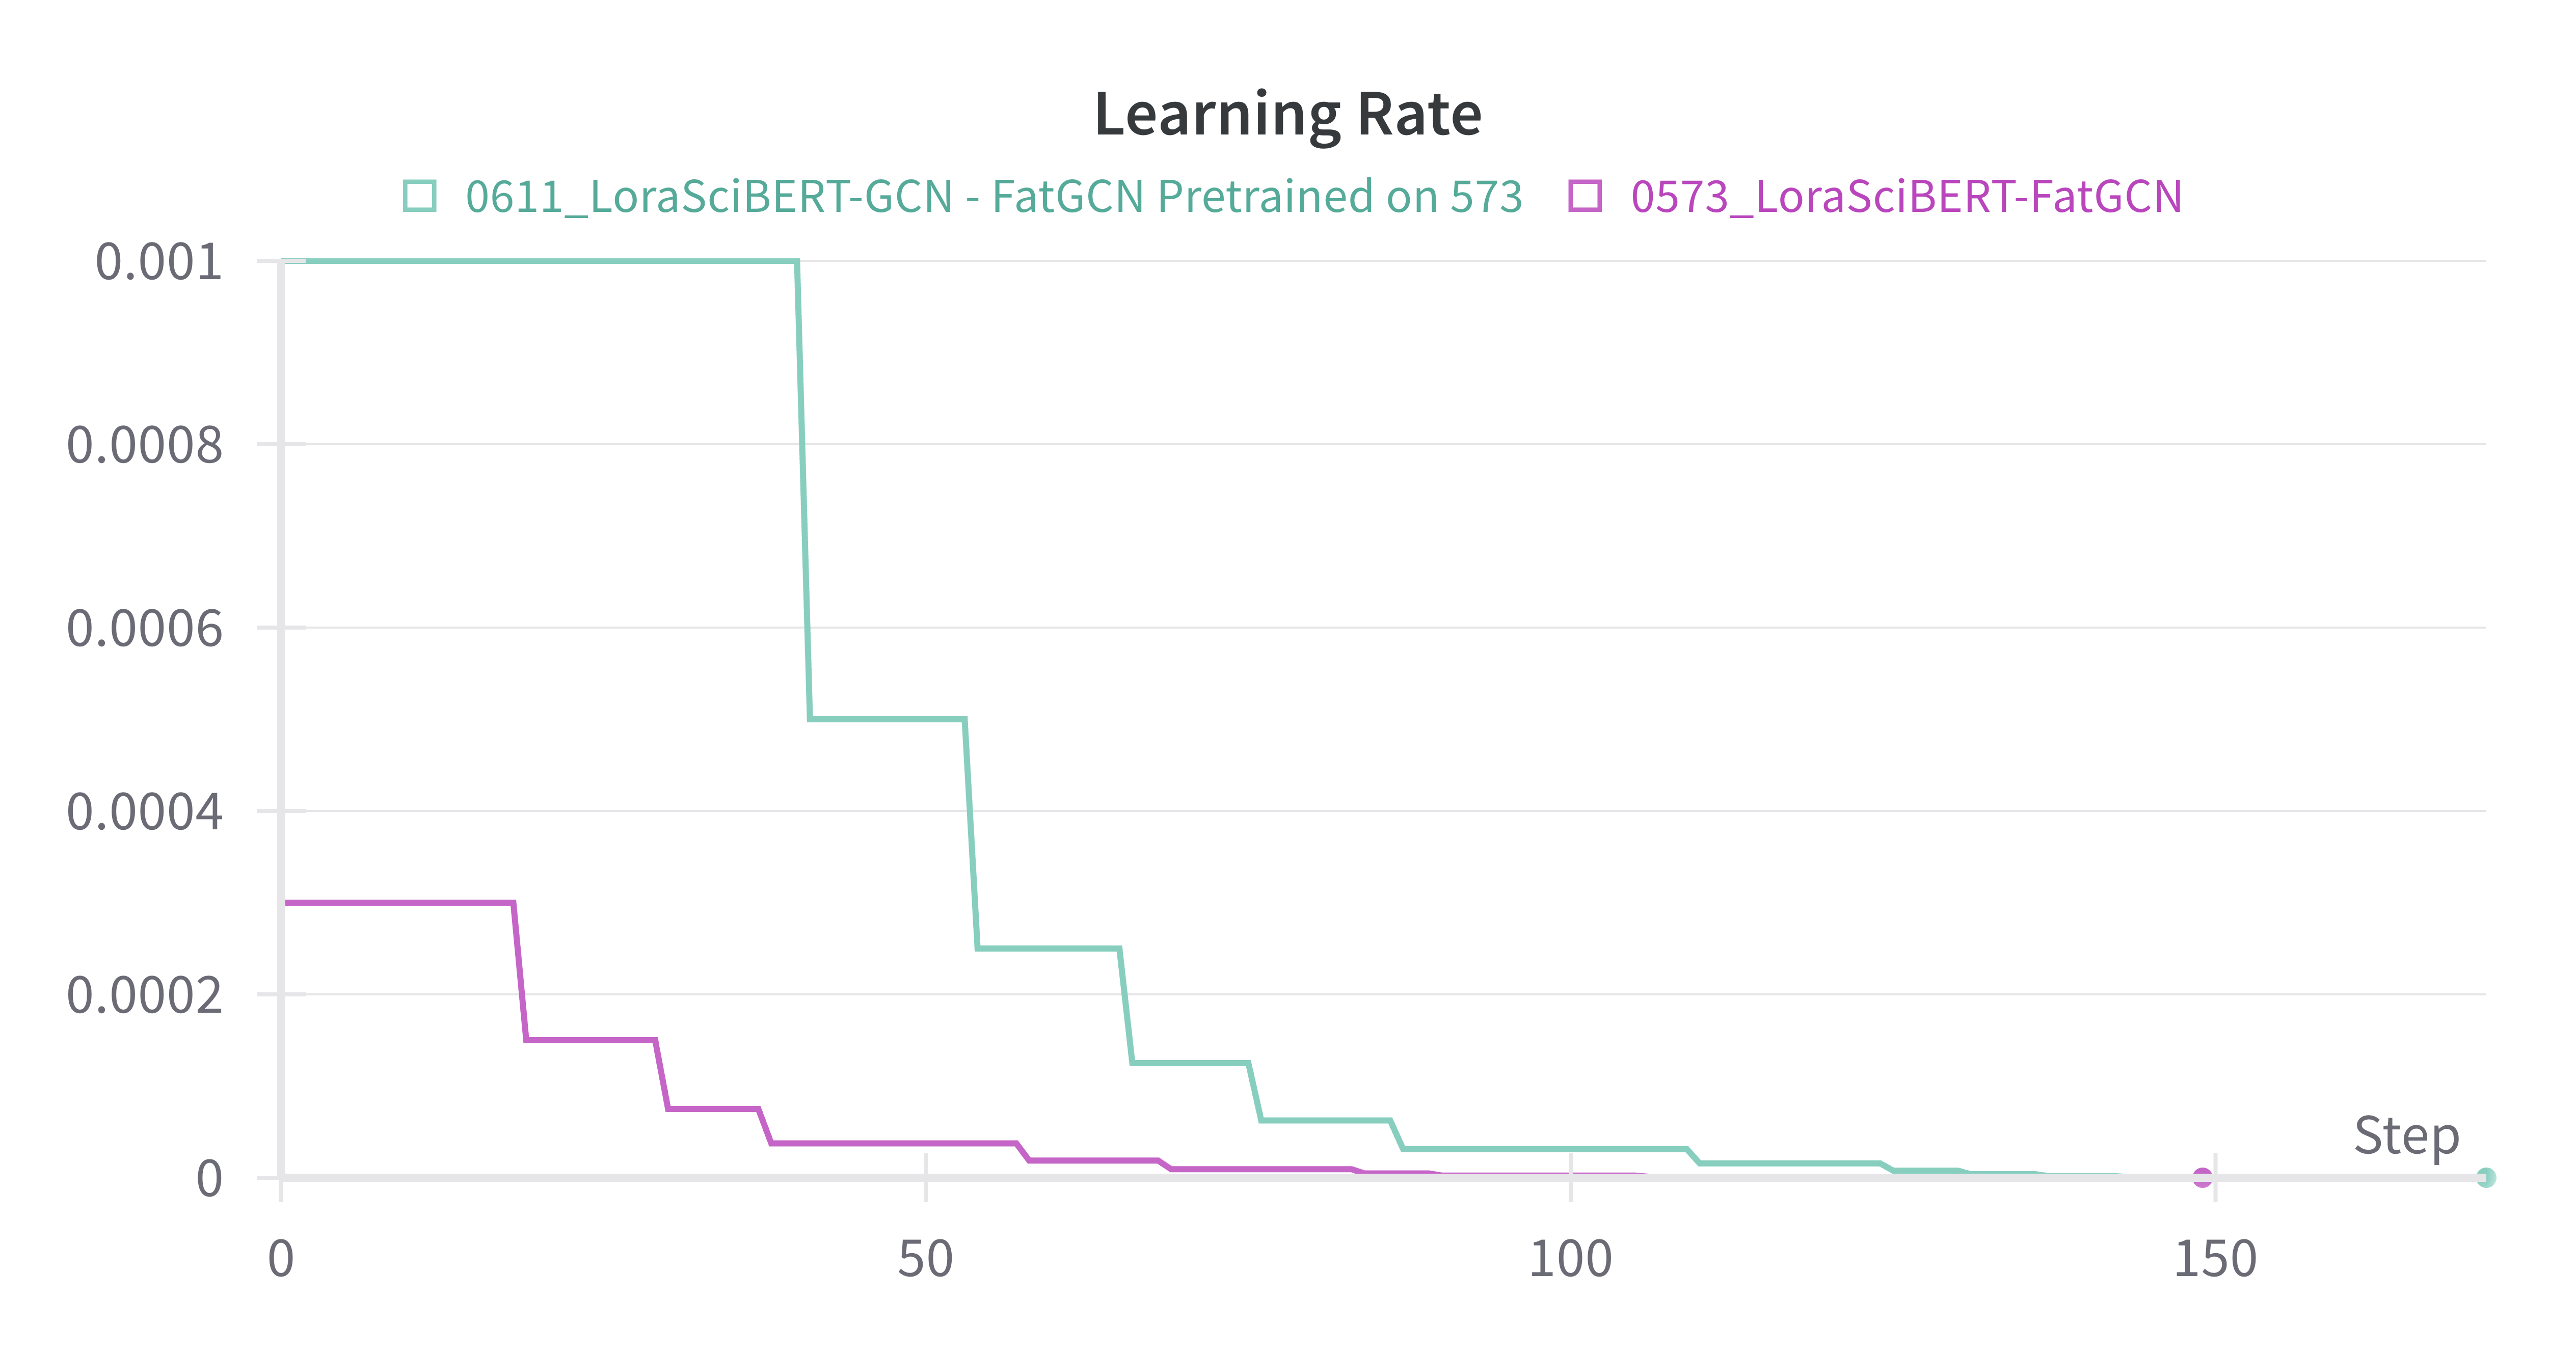
\includegraphics[width=\textwidth]{figures/611_lr.png}
\end{minipage}
\hfill
\begin{minipage}{0.4\textwidth}
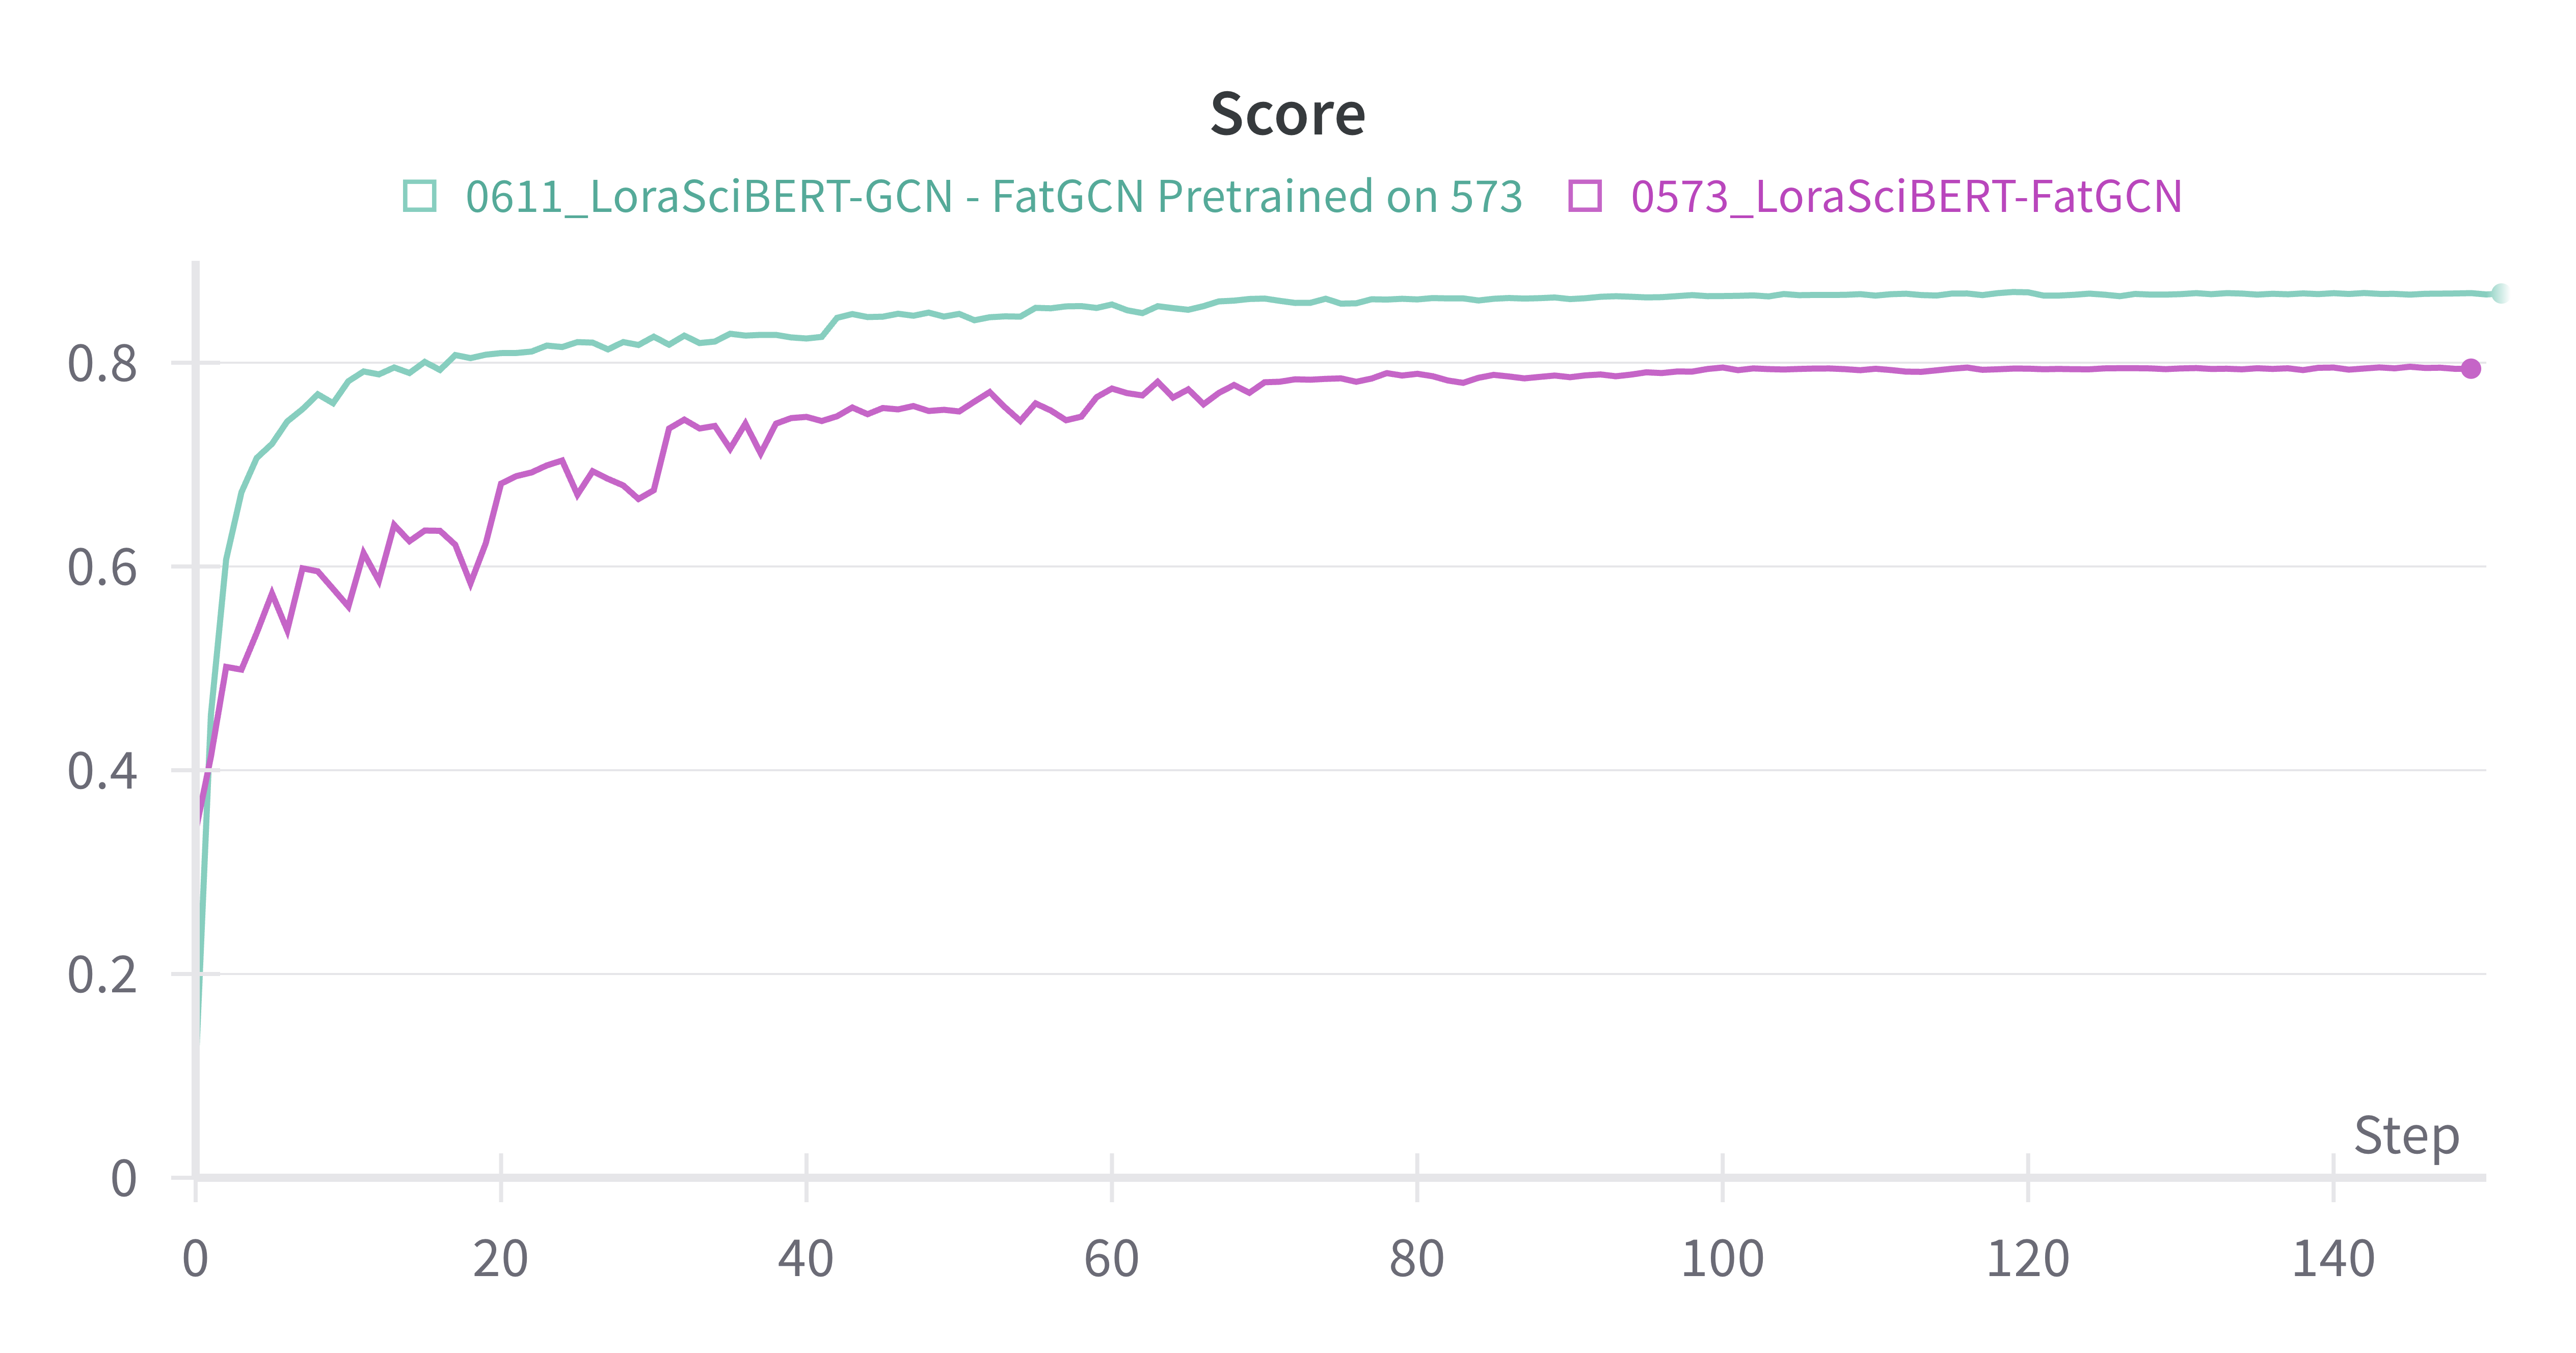
\includegraphics[width=\textwidth]{figures/611_score.png}   
\end{minipage}
\caption{Score and learning rate for fully trained experiment 573 and experiment 611 with frozen LLM}
\label{fig:611}
\end{figure}

% \end{table*}